\scanpage{19}

$G$ groupe d'ordre $60$, opère \inserted{transitivement} sur $I$ ens. d'ordre $15$, sur lequel il y a un autom. $\alpha$ d'ordre $3$ commutant à $G$, d'où $I/\alpha=J$ ens. à $5$ éléments, sur lequel $G$ opère transitivement. Le sous-groupe de stabilité d'un pt \unsure{de|$\in$} $J$ est un sous-groupe \inserted{$F$} d'ordre $12$ de $G$, et on trouve \deleted{que} $G\longrightarrow\unsure{\mathfrak{S}|\mathscr{S}}_5$\inserted{ordre $120$}. Supposons \unsure{pour cela|pour voir|si on sait} que $G$ opère fidèlement sur $J$, alors $G\longrightarrow\mathfrak{S}_5$ est injectif, donc $G\simeq$ sous-groupe d'indice $2$ de $\mathfrak{S}_5$, donc $G\simeq A_5$.

% margin note written sideways
\margin{$\begin{array}{ccc}dD&\longrightarrow&D\\30&&15\\ \alpha'\,?&&\alpha\end{array}$}
% margin note written sideways
\margin{$\alpha'{}^3$ est d'ordre $2$ ou $1$ [\unsure{transfo|transform.} \deleted{\unsure{triviale}} \unsure{correspond} à l'orbite \illegible{2} opposés on a $=$] \par $G/\unsure{H|F|\mathfrak F}_2\longrightarrow G/H_4$}

\figure{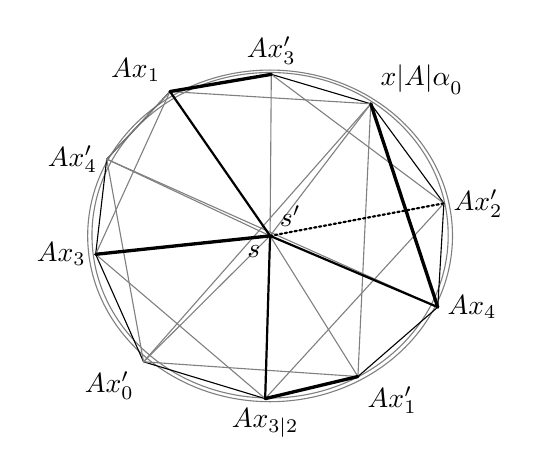
\begin{tikzpicture}[scale=.78,line join=round,line cap=round]
\coordinate (o) at (0,0);
\foreach \nm/\x/\y in {a/1.64/2.15,b/.02/2.63,c/-1.63/2.35,d/-2.66/1.25,e/-2.84/-.30,f/-2.06/-2.05,g/-.08/-2.65,h/1.43/-2.29,i/2.73/-1.16,j/2.83/.53}{\coordinate (\nm) at (\x,\y);}
\draw[gray] (0,0) ellipse (2.97 and 2.70);
\draw[gray] (0,.01) ellipse (2.90 and 2.65);
\draw (a)--(b)--(c)--(d)--(e)--(f)--(g)--(h)--(i)--(j)--cycle;
\draw[gray] (c)--(a)--(h)--(f)--(d)--cycle;
\draw[gray] (b)--(j)--(g)--(e)--(c) (d)--(i) (f)--(a);
\foreach \p in {a,b,d,f,g,h}{\draw[gray] (o)--(\p);}
\draw[thick] (c)--(o)--(i) (o)--(g);
\draw[very thick] (o)--(e) (c)--(b) (a)--(i) (h)--(g);
\draw[densely dotted,thick] (o)--(j);
\node[above right] at (a) {$\unsure{x|A|\alpha}_0$};
\node[above] at (b) {$\deleted{A}x'_3$};
\node[above left] at (c) {$\deleted{A}x_1$};
\node[left] at (d) {$\deleted{A}x'_4$};
\node[left] at (e) {$\deleted{A}x_3$};
\node[below left] at (f) {$\deleted{A}x'_0$};
\node[below] at (g) {$\deleted{A}x_{\unsure{3|2}}$};
\node[below right] at (h) {$\deleted{A}x'_1$};
\node[right] at (i) {$\deleted{A}x_4$};
\node[right] at (j) {$\deleted{A}x'_2$};
\node[below left] at (o) {$s$}; \node[above right] at (o) {$s'$};
\end{tikzpicture}}
\[
 \begin{aligned}
 u&\to u\cos\alpha+v\sin\alpha\\
 v&\to u(-\sin\alpha)+\unsure{v_2|v}\cos\alpha
 \end{aligned}
\]
\figure{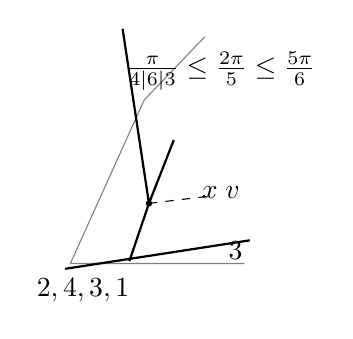
\begin{tikzpicture}[scale=.67]
\draw[thin,gray] (0,0)--(1.4,3.1)--(2.55,4.3) (0,0)--(3.3,0);
\draw[thick] (-.1,-.1)--(3.4,.44) (1.12,.05)--(1.49,1.14)--(1.96,2.34) (1.49,1.14)--(.99,4.45);
\draw[dashed] (1.49,1.14)--(2.74,1.29); \fill (1.49,1.14) circle (.06);
\node[above right] at (.87,3.1) {$\frac{\pi}{\unsure{4|6|3}}\leq\frac{2\pi}{5}\leq\frac{5\pi}{6}$};
\node at (2.85,1.35) {$\deleted{\unsure{x}}\;\unsure{v}$}; \node at (3.13,.25) {$3$};
\node[below] at (.24,-.1) {$2,4,3,1$};
\end{tikzpicture}}
\[
 \alpha'/2=\pi-\tfrac{\alpha}{2}\qquad
 \frac{1}{2\sin^2\theta}-1
\]
\[
 \begin{aligned}
 \cos\alpha&=\cos^2\tfrac{\alpha}{2}-\sin^2\tfrac{\alpha}{2}\\
 &=2\cos^2\tfrac{\alpha}{2}-1\\
 &=1-2\sin^2\theta\\
 &=\cos2\theta
 \end{aligned}
\]
\figure{\begin{tikzpicture}[scale=.56]
\draw (0,0)--(3.9,-.06) (4.2,-.1)--(4.28,2.65) (1.09,.68)--(4.56,1.82);
\node[above] at (2.25,2.03) {$\ell^2=4\sin^2\tfrac{\alpha}{2}$};
\node[rotate=17] at (2.4,1.24) {$2\sin\tfrac{\alpha}{2}\unsure{\cos}$};
\node[right] at (4.2,2.45) {$4$};
\end{tikzpicture}}
\[
 \begin{aligned}
 (AB,A'B')&=P\\
 (EC',CE')&=Q=\alpha(P)\\
 (SD,S'D')&=R=\alpha(Q)=\alpha^2(P)\\
 (AB,A'B')&=\alpha(\unsure{R|P})=\alpha^2(Q)=\alpha^3(P)
 \end{aligned}
\]
\figure{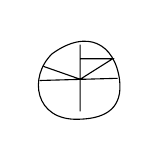
\begin{tikzpicture}[scale=.40]
\draw (0,0) .. controls (-1.4,-.05) and (-1.6,1.35) .. (-.84,2.08) .. controls (.28,2.89) and (1.15,2.39) .. (1.30,1.25) .. controls (1.40,.40) and (.93,.02) .. (0,0);
\draw (.05,.25)--(.05,2.37) (-1.24,1.23)--(1.24,1.30) (-1.12,1.68)--(.05,1.27)--(1.08,1.92)--(.07,1.92);
\end{tikzpicture}}
% margin note written sideways
\margin{$\sigma\in G$, laissant stable $(P,Q,R)$, donc $\sigma\in N$ (\deleted{normalisateur} de Sylow $\simeq\unsure{\mathbb F_2^4|F_2^4}$) l'intersection des conjugués de $N$ est un sous-groupe de $N$, invariant, donc soit $N$, soit $\unsure{\mathbb F|\mathfrak F}_2$, soit $0$. Ce n'est pas $N$, ni $\mathbb F_2$}
% archive sheet number: 18
